\documentclass{ximera}

%% You can put user macros here
%% However, you cannot make new environments

\listfiles

\graphicspath{{./}{firstExample/}{secondExample/}}

\usepackage{tikz}
\usepackage{tkz-euclide}
\usepackage{tikz-3dplot}
\usepackage{tikz-cd}
\usetikzlibrary{shapes.geometric}
\usetikzlibrary{arrows}
\usetikzlibrary{decorations.pathmorphing,patterns}
\usetkzobj{all}
\pgfplotsset{compat=1.13} % prevents compile error.

\renewcommand{\vec}[1]{\mathbf{#1}}
\newcommand{\RR}{\mathbb{R}}
\newcommand{\dfn}{\textit}
\newcommand{\dotp}{\cdot}
\newcommand{\id}{\text{id}}
\newcommand\norm[1]{\left\lVert#1\right\rVert}
 
\newtheorem{general}{Generalization}
\newtheorem{initprob}{Exploration Problem}

\tikzstyle geometryDiagrams=[ultra thick,color=blue!50!black]

\usepackage{mathtools}

\title{Higher Order Constant Coefficients Homogeneous Equations}%\label{Module 7-ADEF}


\begin{document}

\begin{abstract}

\end{abstract}

\maketitle

\section*{Higher Order Constant Coefficients Homogeneous Equations}

If $a_0, a_1, \dots, a_n$ are constants and $a_0\neq 0$, then
$$
a_0y^{(n)}+a_1y^{(n-1)}+\cdots+a_ny=F(x)
$$
is said to be a \dfn{constant coefficient equation}.
In this section we consider the homogeneous constant coefficient
equation
\begin{equation} \label{eq:9.2.1}
a_0y^{(n)}+a_1y^{(n-1)}+\cdots+a_ny=0.
\end{equation}
Since \eqref{eq:9.2.1} is normal on $(-\infty,\infty)$, the theorems in
Section~9.1 all apply with $(a,b)=(-\infty,\infty)$.

As in Section~5.2, we call
\begin{equation} \label{eq:9.2.2}
p(r)=a_0r^n+a_1r^{n-1}+\cdots+a_n
\end{equation}
the \dfn{characteristic polynomial} of \eqref{eq:9.2.1}. We saw in
Section~5.2 that when $n=2$ the solutions of \eqref{eq:9.2.1} are
determined by the zeros of the characteristic polynomial. This is also
true when $n>2$, but the situation is more complicated in this case.
Consequently, we take a different approach here than in
Section~5.2.

If $k$ is a positive integer, let $D^k$ stand
for the $k$-th derivative operator;   that is
$$
D^ky=y^{(k)}.
$$
If
$$
q(r)=b_0r^m+b_1r^{m-1}+\cdots+b_m
$$
is an arbitrary polynomial,  define the operator
$$
q(D)=b_0D^m+b_1D^{m-1}+\cdots+b_m
$$
such that
$$
q(D)y=(b_0D^m+b_1D^{m-1}+\cdots+b_m)y=b_0y^{(m)}+b_1y^{(m-1)}+\cdots+
b_my
$$
whenever $y$ is a function with $m$ derivatives. We call $q(D)$
a \dfn{polynomial}  operator.

With $p$ as in \eqref{eq:9.2.2},
$$
p(D)=a_0D^n+a_1D^{n-1}+\cdots+a_n,
$$
so \eqref{eq:9.2.1} can be written as $p(D)y=0$.  If $r$ is a constant
then
\begin{eqnarray*}
p(D)e^{rx}&=&\left(a_0D^ne^{rx}+a_1D^{n-1}e^{rx}+\cdots+a_ne^{rx}\right)\\
&=&(a_0r^n+a_1r^{n-1}+\cdots+a_n)e^{rx};
\end{eqnarray*}
that is
$$
p(D)(e^{rx})=p(r)e^{rx}.
$$
This shows that $y=e^{rx}$ is a solution of \eqref{eq:9.2.1}
if $p(r)=0$.
In the simplest case, where $p$ has $n$ distinct real zeros
$r_1, r_2,\dots, r_n$, this argument yields $n$ solutions
$$
y_1=e^{r_1x},\quad y_2=e^{r_2x},\dots,\quad y_n=e^{r_nx}.
$$
It can be shown (Exercise~\ref{exer:9.2.39}) that the Wronskian of
$\{e^{r_1x},e^{r_2x},\dots,e^{r_nx}\}$ is nonzero if
$r_1$, $r_2$, \dots, $r_n$ are distinct; hence,
$\{e^{r_1x},e^{r_2x},\dots,e^{r_nx}\}$
is a fundamental set of solutions of $p(D)y=0$ in this case.

\begin{example}\label{example:9.2.1} 
\begin{enumerate}
\item\label{item:9.2.1a} %(a)
Find the general solution of
\begin{equation} \label{eq:9.2.3}
y'''-6y''+11y'-6y=0.
\end{equation}
\item\label{item:9.2.1b} %(b)
Solve the initial value problem
\begin{equation} \label{eq:9.2.4}
y'''-6y''+11y'-6y=0, \quad  y(0)=4,\quad y'(0)=5,\quad y''(0)=9.
\end{equation}
\end{enumerate}


\begin{explanation} \ref{item:9.2.1a} The characteristic polynomial of
\eqref{eq:9.2.3} is
$$
p(r)=r^3-6r^2+11r-6=(r-1)(r-2)(r-3).
$$
Therefore $\{e^x,e^{2x},e^{3x}\}$ is a set of solutions of
\eqref{eq:9.2.3}. It is a fundamental set, since its Wronskian is
$$
W(x)=\begin{vmatrix}e^x&e^{2x}&e^{3x}\\e^x&2e^{2x}&
3e^{3x}\\e^x&4e^{2x}&9e^{3x}\end{vmatrix}=
e^{6x}\begin{vmatrix}1&1&1\\1&2&
3\\1&4&9\end{vmatrix}=2e^{6x}\neq 0.
$$
Therefore the general solution of \eqref{eq:9.2.3} is
\begin{equation} \label{eq:9.2.5}
y=c_1e^{x}+c_2e^{2x}+c_3e^{3x}.
\end{equation}

\ref{item:9.2.1b} We must determine $c_1$, $c_2$ and $c_3$ in
\eqref{eq:9.2.5}
so that $y$ satisfies the initial conditions in \eqref{eq:9.2.4}.
Differentiating \eqref{eq:9.2.5} twice yields
\begin{equation} \label{eq:9.2.6}
\begin{array}{rcl}
y'&=&c_1e^{x}+2c_2e^{2x}+3c_3e^{3x}\\
y''&=&c_1e^{x}+4c_2e^{2x}+9c_3e^{3x}
\end{array}
\end{equation}
Setting $x=0$ in \eqref{eq:9.2.5} and \eqref{eq:9.2.6}  and imposing the
initial conditions yields
$$\begin{array}{rcl}
c_1+c_2+c_3&=&4\\
c_1+2c_2+3c_3&=&5\\
c_1+4c_2+9c_3&=&9.
\end{array}$$
The solution of this system is $c_1=4$, $c_2=-1$, $c_3=1$. Therefore the
solution of \eqref{eq:9.2.4} is
 $$
y=4e^x-e^{2x}+e^{3x}
$$
\begin{image}
 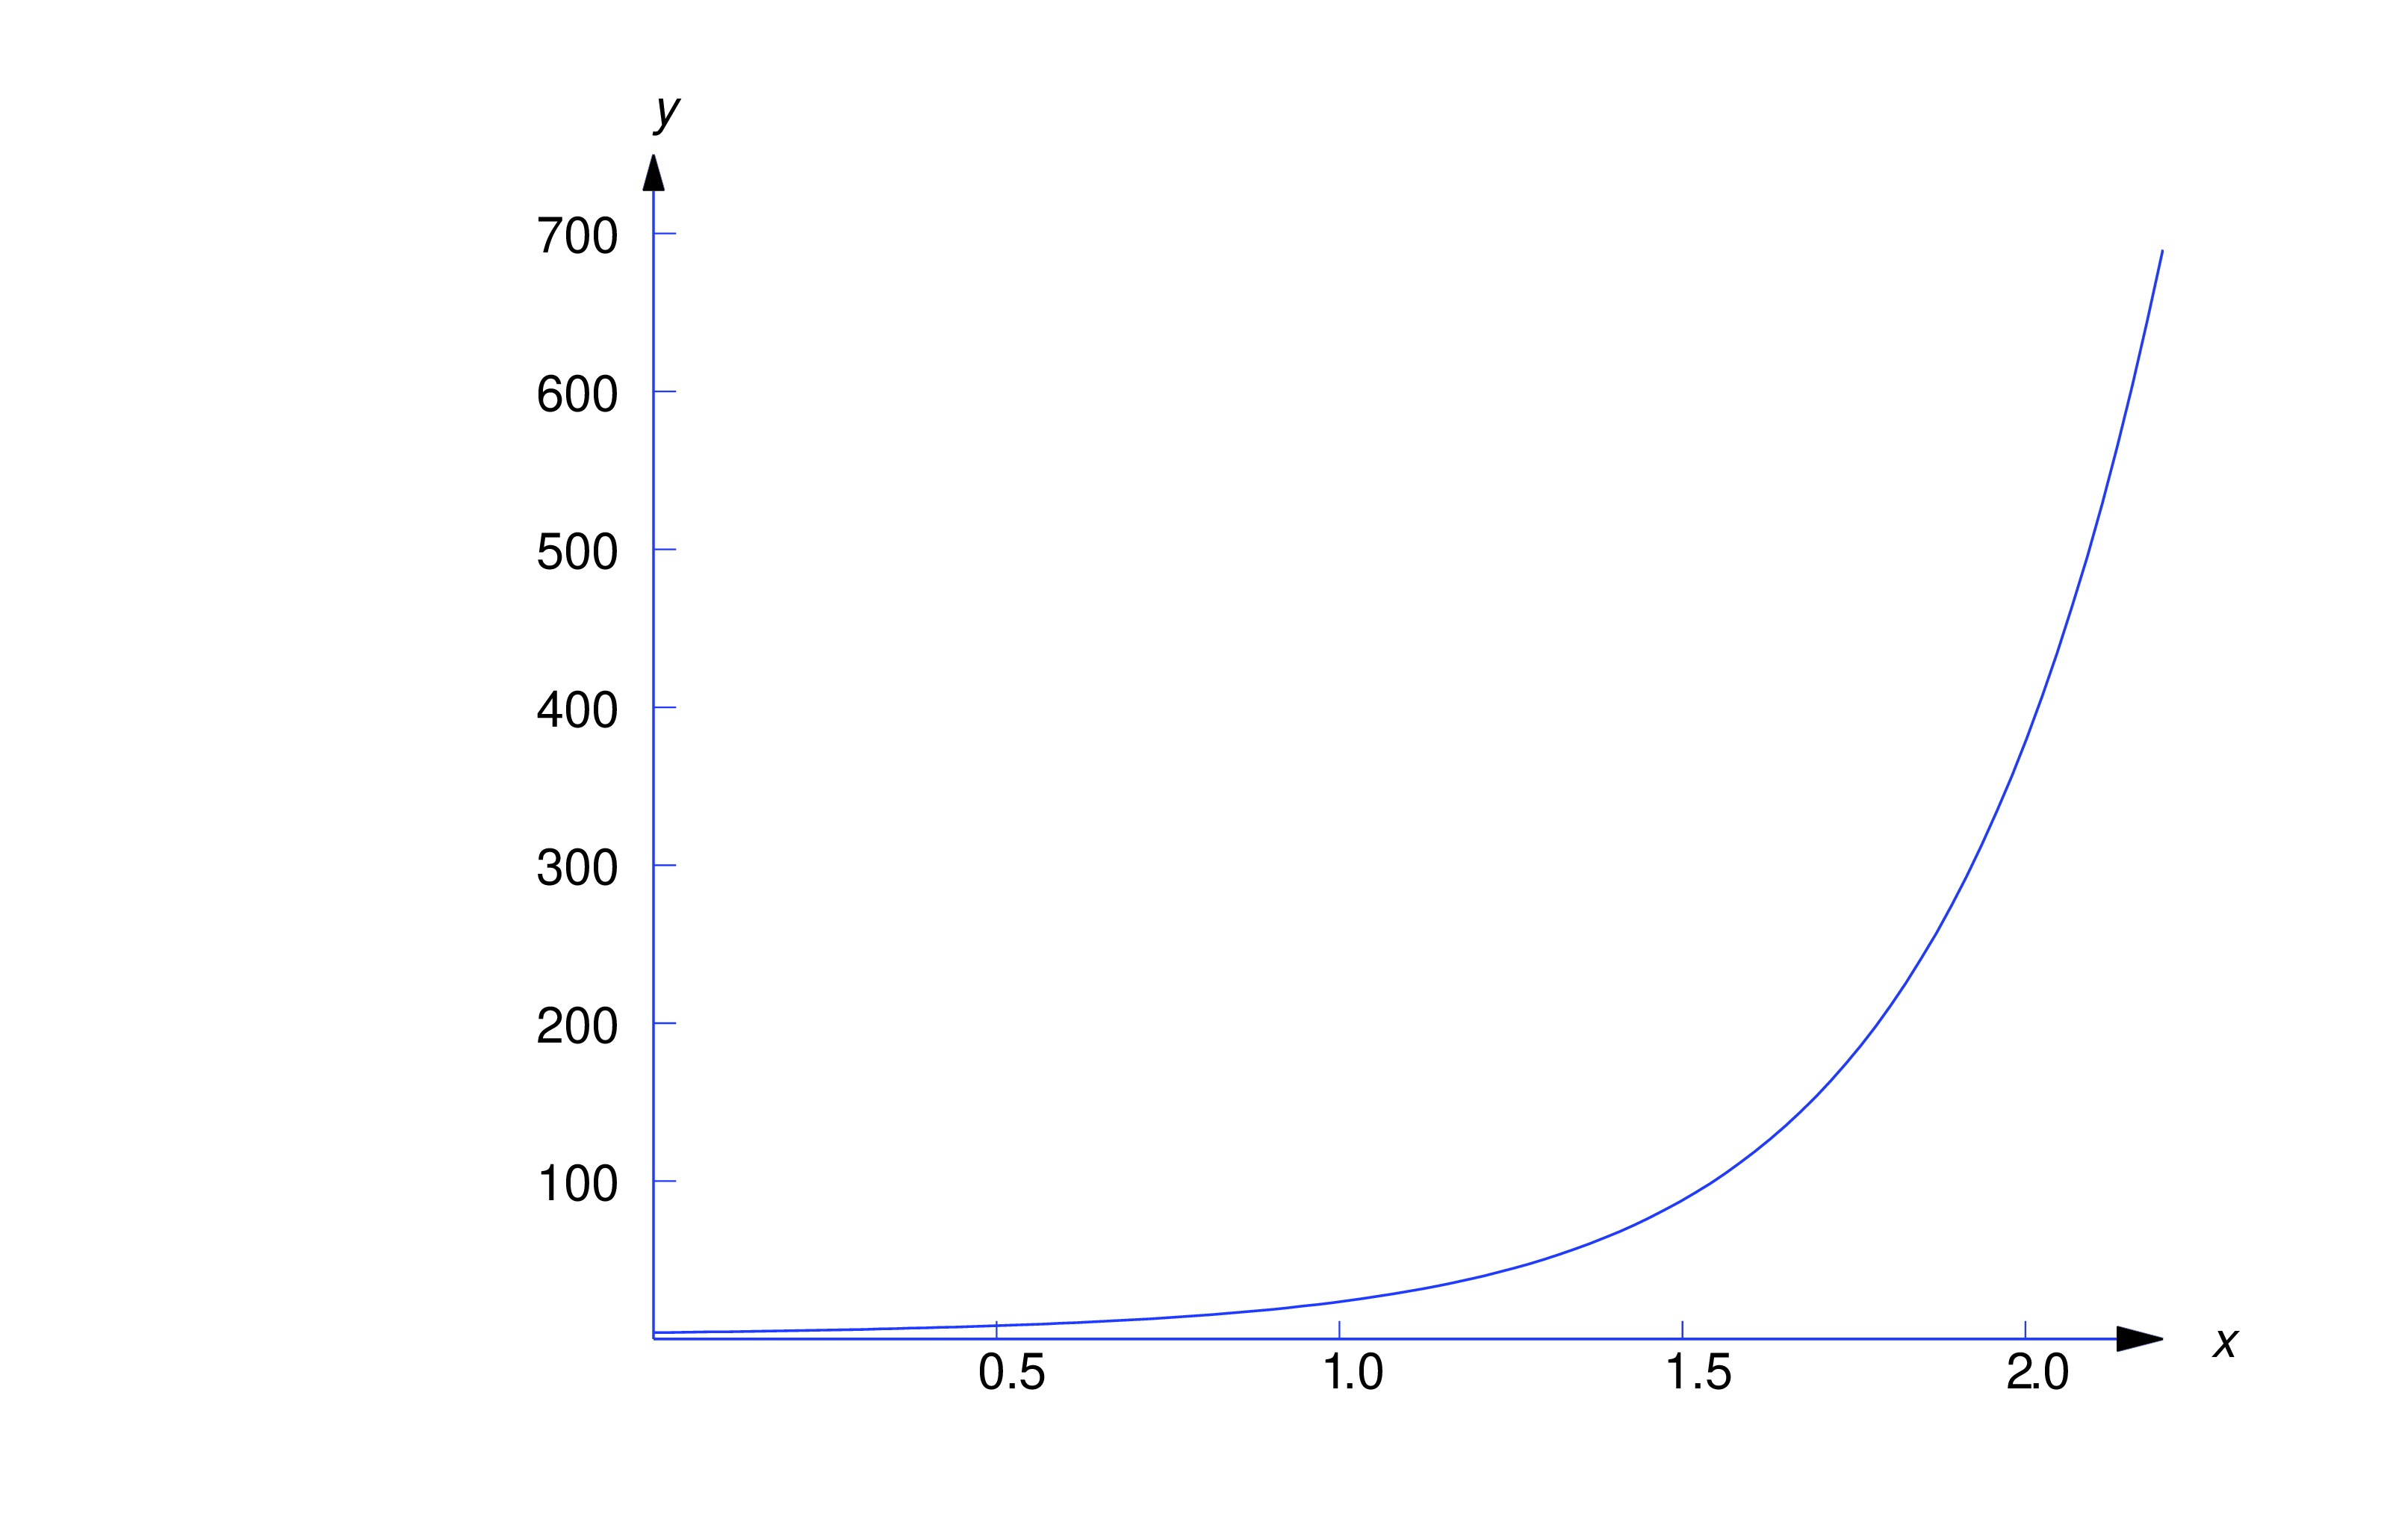
\includegraphics[height=1.5in]{fig090201.jpg} 
\end{image}


\end{explanation}
\end{example}

Now we consider the case where the characteristic polynomial
\eqref{eq:9.2.2} does not have $n$ distinct real zeros. For this purpose
it is useful to define what we mean by a factorization of a polynomial
operator. We begin with an example.

\begin{example}\label{example:9.2.2}
Consider the polynomial
$$
p(r)=r^3-r^2+r-1
$$
and the associated polynomial operator
$$
p(D)=D^3-D^2+D-1.
$$
Since $p(r)$ can be factored as
$$
p(r)=(r-1)(r^2+1)=(r^2+1)(r-1),
$$
it's reasonable to expect that $p(D)$ can be factored as
\begin{equation} \label{eq:9.2.7}
p(D)=(D-1)(D^2+1)=(D^2+1)(D-1).
\end{equation}
However, before we can make this assertion we must define
 what we mean by saying that two operators are equal, and what we mean
by the products of operators in \eqref{eq:9.2.7}. We say that two
operators are equal if they apply to the same functions and always
produce the same result. The definitions of the products in
\eqref{eq:9.2.7} is this: if $y$ is any three-times differentiable
function then
\begin{enumerate}
\item\label{item:9.2.2a} % (a)
$(D-1)(D^2+1)y$
is the function obtained by first applying $D^2+1$ to $y$ and then
applying $D-1$ to the resulting function
\item\label{item:9.2.2b} % (b)
$(D^2+1)(D-1)y$
is the function obtained by first applying $D-1$ to $y$ and then
applying $D^2+1$ to the resulting function.
\end{enumerate}
From \ref{item:9.2.2a},
\begin{equation} \label{eq:9.2.8}
\begin{array}{rcl}
(D-1)(D^2+1)y&=&(D-1)[(D^2+1)y]\\
&=&(D-1)(y''+y)=D(y''+y)-(y''+y)\\&=&(y'''+y')-(y''+y)\\
&=&y'''-y''+y'-y=(D^3-D^2+D-1)y.
\end{array}
\end{equation}
This implies that
$$
(D-1)(D^2+1)=(D^3-D^2+D-1).
$$
From \ref{item:9.2.2b},
\begin{equation} \label{eq:9.2.9}
\begin{array}{rcl}
(D^2+1)(D-1)y&=&(D^2+1)[(D-1)y]\\
&=&(D^2+1)(y'-y)=D^2(y'-y)+(y'-y)\\&=&(y'''-y'')+(y'-y)\\
&=&y'''-y''+y'-y=(D^3-D^2+D-1)y,
\end{array}
\end{equation}
$$
(D^2+1)(D-1)=(D^3-D^2+D-1),
$$
which completes the justification of \eqref{eq:9.2.7}.
\end{example}

\begin{example}\label{example:9.2.3}
Use the result of Example~\ref{example:9.2.2} to find the general
solution of
\begin{equation} \label{eq:9.2.10}
y'''-y''+y'-y=0.
\end{equation}


\begin{explanation}
From \eqref{eq:9.2.8}, we can rewrite \eqref{eq:9.2.10} as
$$
(D-1)(D^2+1)y=0,
$$
which implies that any solution of $(D^2+1)y=0$ is a solution of
\eqref{eq:9.2.10}. Therefore $y_1=\cos x$ and $y_2=\sin x$ are solutions
of \eqref{eq:9.2.10}.


From \eqref{eq:9.2.9}, we can rewrite \eqref{eq:9.2.10} as
$$
(D^2+1)(D-1)y=0,
$$
which implies that any solution of $(D-1)y=0$ is a solution of
\eqref{eq:9.2.10}. Therefore $y_3=e^x$ is solution of \eqref{eq:9.2.10}.

The Wronskian of $\{e^x,\cos x,\sin x\}$ is
$$
W(x)=\begin{vmatrix}\cos x&\sin x&e^x\\-\sin x&\cos x&e^x\\
-\cos x&-\sin x&e^x\end{vmatrix}.
$$
Since
$$
W(0)=\begin{vmatrix}1&0&1\\0&1&1\\
-1&0&1\end{vmatrix}=2,
$$
 $\{\cos x,\sin x,e^x\}$ is linearly independent
and
$$
y=c_1\cos x+c_2\sin x+c_3e^x
$$
is the general solution of \eqref{eq:9.2.10}.
\end{explanation}
\end{example}

\begin{example}\label{example:9.2.4}
Find the general solution of
\begin{equation} \label{eq:9.2.11}
y^{(4)}-16y=0.
\end{equation}


\begin{explanation}
The characteristic polynomial of
\eqref{eq:9.2.11} is
$$
p(r)=r^4-16=(r^2-4)(r^2+4)=(r-2)(r+2)(r^2+4).
$$
By arguments similar to those used in Examples~\ref{example:9.2.2} and
\ref{example:9.2.3}, it can be shown that \eqref{eq:9.2.11} can be written
as
$$
(D^2+4)(D+2)(D-2)y=0
$$
or
$$
(D^2+4)(D-2)(D+2)y=0
$$
or
$$
(D-2)(D+2)(D^2+4)y=0.
$$
Therefore $y$  is a solution of \eqref{eq:9.2.11} if it's a solution
of any  of the three  equations
$$
 (D-2)y=0,\quad (D+2)y=0, \quad(D^2+4)y=0.
$$
Hence, $\{e^{2x},e^{-2x},\cos2x,\sin2x\}$ is a set of solutions of
\eqref{eq:9.2.11}. The Wronskian of this set is
$$
W(x)=\begin{vmatrix}
e^{2x}&e^{-2x}&\cos2x&\sin2x\\
2e^{2x}&-2e^{-2x}&-2\sin2x&2\cos2x\\
4e^{2x}&4e^{-2x}&-4\cos2x&-4\sin2x\\
8e^{2x}&-8e^{-2x}&8\sin2x&-8\cos2x\\
\end{vmatrix}.
$$
Since
$$
W(0)=\begin{vmatrix}
1&1&1&0\\
2&-2&0&2\\
4&4&-4&0\\
8&-8&0&-8\\
\end{vmatrix}=-512,
$$
 $\{e^{2x},e^{-2x},\cos2x,\sin2x\}$ is linearly independent,
and
$$
y_1=c_1e^{2x}+c_2e^{-2x}+c_3\cos2x+c_4\sin2x
$$
is   the general solution of \eqref{eq:9.2.11}.
\end{explanation}
\end{example}

It is known from algebra that every polynomial
$$
p(r)=a_0r^n+a_1r^{n-1}+\cdots+a_n
$$
with real coefficients can be factored as
$$
p(r)=a_0p_1(r)p_2(r)\cdots p_k(r),
$$
where no pair of the polynomials $p_1, p_2, \dots, p_k$  has a common
factor and each  is either of the form
\begin{equation} \label{eq:9.2.12}
p_j(r)=(r-r_j)^{m_j},
\end{equation}
where $r_j$ is real and $m_j$ is a positive integer, or
\begin{equation} \label{eq:9.2.13}
p_j(r)=\left[(r-\lambda_j)^2+\omega_j^2\right]^{m_j},
\end{equation}
where $\lambda_j$ and $\omega_j$ are real, $\omega_j\neq 0$, and $m_j$
is a positive integer. If \eqref{eq:9.2.12} holds then $r_j$ is a real
zero of $p$, while if \eqref{eq:9.2.13} holds then $\lambda+i\omega$
and $\lambda-i\omega$ are complex conjugate zeros of $p$. In either
case, $m_j$ is the \dfn{multiplicity} of the zero(s).


By arguments similar to those used in our examples, it can be shown
that
\begin{equation} \label{eq:9.2.14}
p(D)=a_0p_1(D)p_2(D)\cdots p_k(D)
\end{equation}
and that the order of the factors on the right can be chosen
arbitrarily. Therefore, if $p_j(D)y=0$ for some $j$ then
$p(D)y=0$. To see this, we simply rewrite \eqref{eq:9.2.14} so that
$p_j(D)$ is applied first. Therefore the problem of finding solutions
of $p(D)y=0$ with $p$ as in \eqref{eq:9.2.14} reduces to finding solutions
of each of these equations
$$
p_j(D)y=0,\quad 1\leq j\leq k,
$$
where $p_j$ is a power of a first degree term or of an irreducible
quadratic. To find a fundamental set of solutions
$\{y_1,y_2,\dots,y_n\}$ of $p(D)y=0$, we find fundamental set of
solutions of each of the equations and take $\{y_1,y_2,\dots,y_n\}$ to
be the set of all functions in these separate fundamental sets. In
Exercise~\ref{exer:9.2.40} we sketch the proof that
$\{y_1,y_2,\dots,y_n\}$ is linearly independent, and therefore a
fundamental set of solutions of $p(D)y=0$.

To apply this procedure to general homogeneous constant coefficient
equations, we must be able to find fundamental sets of solutions of
equations of the form
$$
(D-a)^my=0
$$
and
$$
\left[(D-\lambda)^2+\omega^2\right]^my=0,
$$
where $m$ is an arbitrary positive integer. The next two theorems show
how to do this.

\begin{theorem}\label{thmtype:9.2.1}
If $m$ is a positive integer, then
\begin{equation} \label{eq:9.2.15}
\{e^{ax}, xe^{ax},\dots, x^{m-1}e^{ax}\}
\end{equation}
is a fundamental set of solutions of
\begin{equation} \label{eq:9.2.16}
(D-a)^my=0.
\end{equation}
\end{theorem}

\begin{proof}
We'll show that if
$$
f(x)=c_1+c_2x+\cdots+c_mx^{m-1}
$$
is an arbitrary polynomial of degree $\le m-1$, then $y=e^{ax}f$
is a solution of \eqref{eq:9.2.16}. First note that if $g$ is any
differentiable function then
$$
(D-a)e^{ax}g=De^{ax}g-ae^{ax}g=ae^{ax}g+e^{ax}g'-ae^{ax}g,
$$
so
\begin{equation} \label{eq:9.2.17}
(D-a)e^{ax}g=e^{ax}g'.
\end{equation}
Therefore
$$
\begin{array}{lcll}
(D-a)e^{ax}f&=&e^{ax}f'&\mbox{(from \eqref{eq:9.2.17} with
$g=f$)}\\
(D-a)^2e^{ax}f&=&
(D-a)e^{ax}f'=e^{ax}f''
&\mbox{(from \eqref{eq:9.2.17} with $g=f'$)}\\
(D-a)^3e^{ax}f&=&
(D-a)e^{ax}f''=e^{ax}f'''
&\mbox{(from \eqref{eq:9.2.17} with $g=f''$)}\\
&\vdots&\\
(D-a)^me^{ax}f
&=&(D-a)e^{ax}f^{(m-1)}=e^{ax}f^{(m)}
&\mbox{(from \eqref{eq:9.2.17} with $g=f^{(m-1)}$)}.
\end{array}
$$
Since $f^{(m)}=0$, the last equation implies that $y=e^{ax}f$ is a
solution of \eqref{eq:9.2.16} if $f$ is any polynomial of degree $\leq
m-1$. In particular, each function in \eqref{eq:9.2.15} is a solution of
\eqref{eq:9.2.16}. To see that \eqref{eq:9.2.15} is linearly independent (and
therefore a fundamental set of solutions of \eqref{eq:9.2.16}), note that
if
$$
c_1e^{ax}+c_2xe^{ax}+c\dots+c_{m-1}x^{m-1}e^{ax}=0
$$
for all $x$ in some interval $(a,b)$, then
$$
c_1+c_2x+c\dots+c_{m-1}x^{m-1}=0
$$
for all $x$ in $(a,b)$.  However, we know from algebra that if this
polynomial has more than $m-1$ zeros then $c_1=c_2=\cdots=c_n=0$.
\end{proof}

\begin{example}\label{example:9.2.5}
Find the general solution of
\begin{equation} \label{eq:9.2.18}
y'''+3y''+3y'+y=0.
\end{equation}


\begin{explanation} The characteristic polynomial of \eqref{eq:9.2.18} is
$$
p(r)=r^3+3r^2+3r+1=(r+1)^3.
$$
Therefore \eqref{eq:9.2.18} can be written as
$$
(D+1)^3y=0,
$$
so Theorem~\ref{thmtype:9.2.1} implies that the general solution of
\eqref{eq:9.2.18} is
$$
y=e^{-x}(c_1+c_2x+c_3x^2).
$$
\end{explanation}
\end{example}

The proof of the next theorem is sketched in
Exercise~\ref{exer:9.2.41}.

\begin{theorem}\label{thmtype:9.2.2}
If $\omega \neq 0$ and $m$ is a positive integer, then
$$
\begin{array}{rl}
\{e^{\lambda x}\cos\omega x, xe^{\lambda x}\cos\omega x,
&\dots, x^{m-1}e^{\lambda x}\cos\omega x,\\
e^{\lambda x}\sin\omega x, xe^{\lambda x}\sin\omega x,&
\dots, x^{m-1}e^{\lambda x}\sin\omega x\}
\end{array}
$$
is a fundamental set of solutions of
$$
[(D-\lambda)^2+\omega^2]^my=0.
$$
\end{theorem}

\begin{example}\label{example:9.2.6}
Find the general solution of
\begin{equation} \label{eq:9.2.19}
(D^2+4D+13)^3y=0.
\end{equation}


\begin{explanation}  The characteristic polynomial of \eqref{eq:9.2.19} is
$$
p(r)=(r^2+4r+13)^3=\left((r+2)^2+9\right)^3.
$$
Therefore \eqref{eq:9.2.19} can be be written as
$$
[(D+2)^2+9]^3y=0,
$$
so Theorem~\ref{thmtype:9.2.2} implies that the general solution of
\eqref{eq:9.2.19} is
$$
y=(a_1+a_2x+a_3x^2)e^{-2x}\cos3x
+(b_1+b_2x+b_3x^2)e^{-2x}\sin3x.
$$
\end{explanation}
\end{example}

\begin{example}\label{example:9.2.7}
Find the general solution of
\begin{equation} \label{eq:9.2.20}
y^{(4)}+4y'''+6y''+4y'=0.
\end{equation}


\begin{explanation}  The characteristic polynomial of \eqref{eq:9.2.20} is
\begin{eqnarray*}
p(r)&=&r^4+4r^3+6r^2+4r\\
&=&r(r^3+4r^2+6r+4)\\
&=&r(r+2)(r^2+2r+2)\\
&=&r(r+2)[(r+1)^2+1].
\end{eqnarray*}
Therefore \eqref{eq:9.2.20} can be written as
$$
[(D+1)^2+1](D+2)Dy=0.
$$
Fundamental sets of solutions of
$$
\left[(D+1)^2+1\right] y=0,\quad (D+2) y=0,\quad\mbox{and}\quad Dy=0.
$$
are given by
$$
\{e^{-x}\cos x,e^{-x}\sin x\},\quad \{e^{-2x}\},\quad\mbox{and}\quad \{1\},
$$
respectively. Therefore the general solution of \eqref{eq:9.2.20} is
$$
y=e^{-x}(c_1\cos x+c_2\sin x)+c_3e^{-2x}+c_4.
$$
\end{explanation}
\end{example}

\begin{example}\label{example:9.2.8}
Find a fundamental set of solutions of
\begin{equation} \label{eq:9.2.21}
[(D+1)^2+1]^2(D-1)^3(D+1)D^2y=0.
\end{equation}


\begin{explanation} A fundamental set of solutions of \eqref{eq:9.2.21} can be
obtained by combining fundamental sets of solutions of
$$
\begin{array}{c}
\left[(D+1)^2+1\right]^2 y=0,\quad (D-1)^3 y=0,\\
(D+1)y=0,\quad \mbox{and} \quad D^2y=0.
\end{array}
$$
Fundamental sets of solutions of these equations are given by
$$
\begin{array}{c}
\{e^{-x}\cos x, xe^{-x}\cos x, e^{-x}\sin x, xe^{-x}\sin
x\},\quad \{e^x, xe^x, x^2e^x\},\\
\{e^{-x}\},\mbox{and} \{1,x\},
\end{array}
$$
respectively. These ten functions form a fundamental set of solutions
of \eqref{eq:9.2.21}.
\end{explanation}
\end{example}


\section*{Text Source}
Trench, William F., "Elementary Differential Equations" (2013). Faculty Authored and Edited Books \& CDs. 8. (CC-BY-NC-SA)

\href{https://digitalcommons.trinity.edu/mono/8/}{https://digitalcommons.trinity.edu/mono/8/}


\end{document}